% Created by tikzDevice version 0.11 on 2018-04-09 15:27:55
% !TEX encoding = UTF-8 Unicode
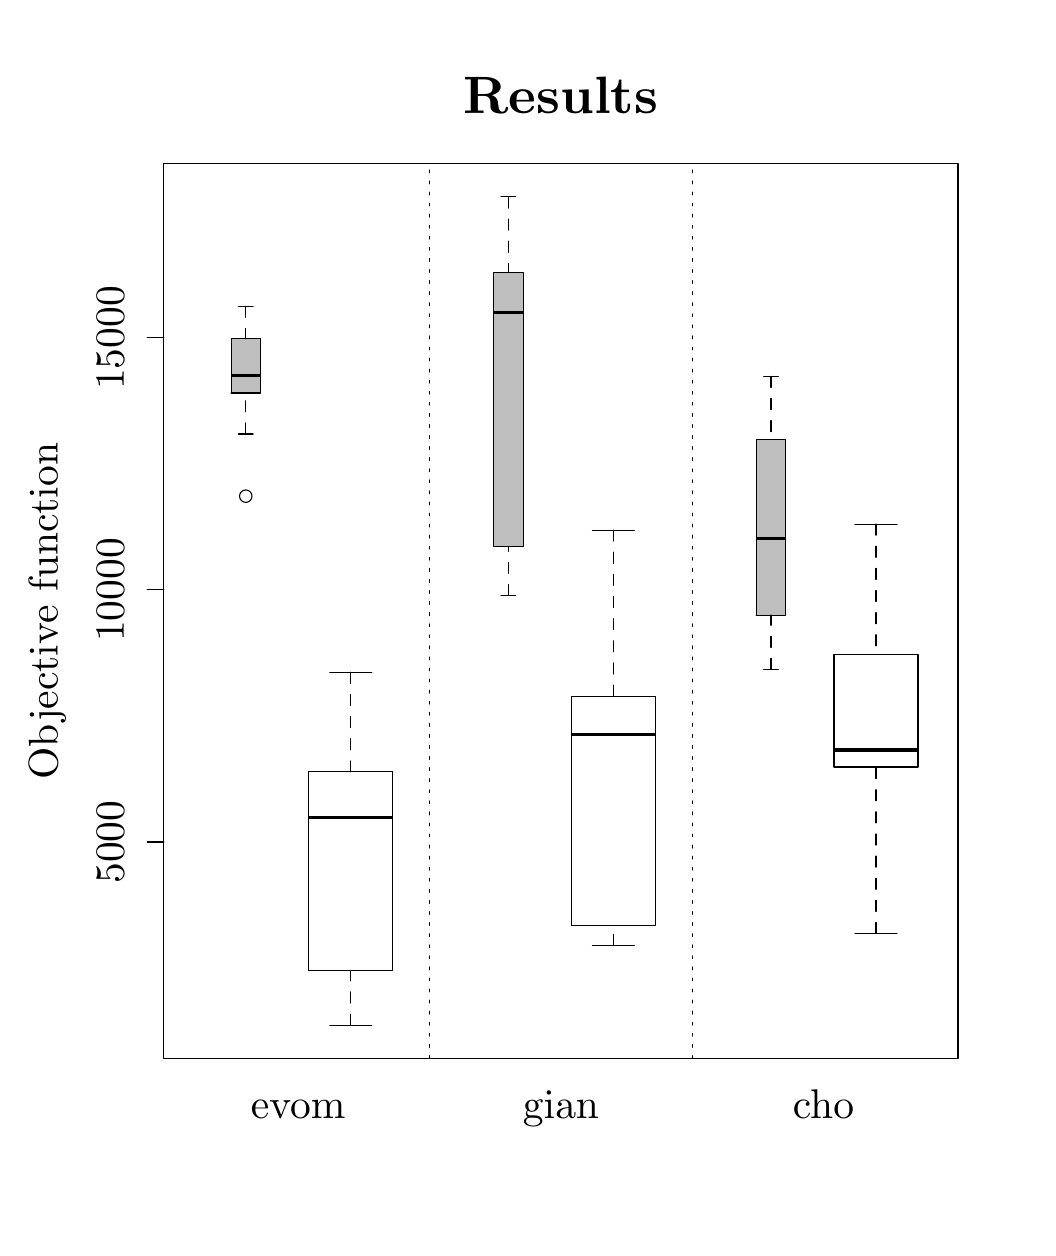
\begin{tikzpicture}[x=1pt,y=1pt]
\definecolor{fillColor}{RGB}{255,255,255}
\path[use as bounding box,fill=fillColor,fill opacity=0.00] (0,0) rectangle (361.35,433.62);
\begin{scope}
\path[clip] ( 49.20, 61.20) rectangle (336.15,384.42);
\definecolor{fillColor}{RGB}{190,190,190}

\path[fill=fillColor] ( 73.49,301.62) --
	( 84.12,301.62) --
	( 84.12,321.17) --
	( 73.49,321.17) --
	cycle;
\definecolor{drawColor}{RGB}{0,0,0}

\path[draw=drawColor,line width= 1.2pt,line join=round] ( 73.49,307.98) -- ( 84.12,307.98);

\path[draw=drawColor,line width= 0.4pt,dash pattern=on 4pt off 4pt ,line join=round,line cap=round] ( 78.81,286.79) -- ( 78.81,301.62);

\path[draw=drawColor,line width= 0.4pt,dash pattern=on 4pt off 4pt ,line join=round,line cap=round] ( 78.81,332.92) -- ( 78.81,321.17);

\path[draw=drawColor,line width= 0.4pt,line join=round,line cap=round] ( 76.15,286.79) -- ( 81.46,286.79);

\path[draw=drawColor,line width= 0.4pt,line join=round,line cap=round] ( 76.15,332.92) -- ( 81.46,332.92);

\path[draw=drawColor,line width= 0.4pt,line join=round,line cap=round] ( 73.49,301.62) --
	( 84.12,301.62) --
	( 84.12,321.17) --
	( 73.49,321.17) --
	( 73.49,301.62);

\path[draw=drawColor,line width= 0.4pt,line join=round,line cap=round] ( 78.81,264.33) circle (  2.25);
\definecolor{fillColor}{RGB}{255,255,255}

\path[fill=fillColor] (101.58, 92.86) --
	(131.94, 92.86) --
	(131.94,164.70) --
	(101.58,164.70) --
	cycle;

\path[draw=drawColor,line width= 1.2pt,line join=round] (101.58,148.13) -- (131.94,148.13);

\path[draw=drawColor,line width= 0.4pt,dash pattern=on 4pt off 4pt ,line join=round,line cap=round] (116.76, 73.17) -- (116.76, 92.86);

\path[draw=drawColor,line width= 0.4pt,dash pattern=on 4pt off 4pt ,line join=round,line cap=round] (116.76,200.69) -- (116.76,164.70);

\path[draw=drawColor,line width= 0.4pt,line join=round,line cap=round] (109.17, 73.17) -- (124.35, 73.17);

\path[draw=drawColor,line width= 0.4pt,line join=round,line cap=round] (109.17,200.69) -- (124.35,200.69);

\path[draw=drawColor,line width= 0.4pt,line join=round,line cap=round] (101.58, 92.86) --
	(131.94, 92.86) --
	(131.94,164.70) --
	(101.58,164.70) --
	(101.58, 92.86);
\definecolor{fillColor}{RGB}{190,190,190}

\path[fill=fillColor] (168.38,246.18) --
	(179.01,246.18) --
	(179.01,345.21) --
	(168.38,345.21) --
	cycle;

\path[draw=drawColor,line width= 1.2pt,line join=round] (168.38,330.69) -- (179.01,330.69);

\path[draw=drawColor,line width= 0.4pt,dash pattern=on 4pt off 4pt ,line join=round,line cap=round] (173.70,228.40) -- (173.70,246.18);

\path[draw=drawColor,line width= 0.4pt,dash pattern=on 4pt off 4pt ,line join=round,line cap=round] (173.70,372.45) -- (173.70,345.21);

\path[draw=drawColor,line width= 0.4pt,line join=round,line cap=round] (171.04,228.40) -- (176.35,228.40);

\path[draw=drawColor,line width= 0.4pt,line join=round,line cap=round] (171.04,372.45) -- (176.35,372.45);

\path[draw=drawColor,line width= 0.4pt,line join=round,line cap=round] (168.38,246.18) --
	(179.01,246.18) --
	(179.01,345.21) --
	(168.38,345.21) --
	(168.38,246.18);
\definecolor{fillColor}{RGB}{255,255,255}

\path[fill=fillColor] (196.47,109.13) --
	(226.84,109.13) --
	(226.84,191.95) --
	(196.47,191.95) --
	cycle;

\path[draw=drawColor,line width= 1.2pt,line join=round] (196.47,178.25) -- (226.84,178.25);

\path[draw=drawColor,line width= 0.4pt,dash pattern=on 4pt off 4pt ,line join=round,line cap=round] (211.65,101.94) -- (211.65,109.13);

\path[draw=drawColor,line width= 0.4pt,dash pattern=on 4pt off 4pt ,line join=round,line cap=round] (211.65,252.07) -- (211.65,191.95);

\path[draw=drawColor,line width= 0.4pt,line join=round,line cap=round] (204.06,101.94) -- (219.24,101.94);

\path[draw=drawColor,line width= 0.4pt,line join=round,line cap=round] (204.06,252.07) -- (219.24,252.07);

\path[draw=drawColor,line width= 0.4pt,line join=round,line cap=round] (196.47,109.13) --
	(226.84,109.13) --
	(226.84,191.95) --
	(196.47,191.95) --
	(196.47,109.13);
\definecolor{fillColor}{RGB}{190,190,190}

\path[fill=fillColor] (263.27,221.33) --
	(273.90,221.33) --
	(273.90,284.75) --
	(263.27,284.75) --
	cycle;

\path[draw=drawColor,line width= 1.2pt,line join=round] (263.27,249.04) -- (273.90,249.04);

\path[draw=drawColor,line width= 0.4pt,dash pattern=on 4pt off 4pt ,line join=round,line cap=round] (268.59,201.68) -- (268.59,221.33);

\path[draw=drawColor,line width= 0.4pt,dash pattern=on 4pt off 4pt ,line join=round,line cap=round] (268.59,307.63) -- (268.59,284.75);

\path[draw=drawColor,line width= 0.4pt,line join=round,line cap=round] (265.93,201.68) -- (271.24,201.68);

\path[draw=drawColor,line width= 0.4pt,line join=round,line cap=round] (265.93,307.63) -- (271.24,307.63);

\path[draw=drawColor,line width= 0.4pt,line join=round,line cap=round] (263.27,221.33) --
	(273.90,221.33) --
	(273.90,284.75) --
	(263.27,284.75) --
	(263.27,221.33);
\definecolor{fillColor}{RGB}{255,255,255}

\path[fill=fillColor] (291.36,166.46) --
	(321.73,166.46) --
	(321.73,207.22) --
	(291.36,207.22) --
	cycle;

\path[draw=drawColor,line width= 1.2pt,line join=round] (291.36,172.64) -- (321.73,172.64);

\path[draw=drawColor,line width= 0.4pt,dash pattern=on 4pt off 4pt ,line join=round,line cap=round] (306.54,106.27) -- (306.54,166.46);

\path[draw=drawColor,line width= 0.4pt,dash pattern=on 4pt off 4pt ,line join=round,line cap=round] (306.54,254.24) -- (306.54,207.22);

\path[draw=drawColor,line width= 0.4pt,line join=round,line cap=round] (298.95,106.27) -- (314.14,106.27);

\path[draw=drawColor,line width= 0.4pt,line join=round,line cap=round] (298.95,254.24) -- (314.14,254.24);

\path[draw=drawColor,line width= 0.4pt,line join=round,line cap=round] (291.36,166.46) --
	(321.73,166.46) --
	(321.73,207.22) --
	(291.36,207.22) --
	(291.36,166.46);
\end{scope}
\begin{scope}
\path[clip] (  0.00,  0.00) rectangle (361.35,433.62);
\definecolor{drawColor}{RGB}{0,0,0}

\node[text=drawColor,rotate= 90.00,anchor=base,inner sep=0pt, outer sep=0pt, scale=  1.50] at ( 10.80,222.81) {Objective function};
\end{scope}
\begin{scope}
\path[clip] ( 49.20, 61.20) rectangle (336.15,384.42);
\definecolor{drawColor}{RGB}{0,0,0}

\path[draw=drawColor,line width= 0.4pt,dash pattern=on 1pt off 3pt ,line join=round,line cap=round] (145.23, 61.20) -- (145.23,384.42);

\path[draw=drawColor,line width= 0.4pt,dash pattern=on 1pt off 3pt ,line join=round,line cap=round] (240.12, 61.20) -- (240.12,384.42);
\end{scope}
\begin{scope}
\path[clip] (  0.00,  0.00) rectangle (361.35,433.62);
\definecolor{drawColor}{RGB}{0,0,0}

\node[text=drawColor,anchor=base,inner sep=0pt, outer sep=0pt, scale=  1.50] at ( 97.78, 39.60) {evom};

\node[text=drawColor,anchor=base,inner sep=0pt, outer sep=0pt, scale=  1.50] at (192.67, 39.60) {gian};

\node[text=drawColor,anchor=base,inner sep=0pt, outer sep=0pt, scale=  1.50] at (287.57, 39.60) {cho};
\end{scope}
\begin{scope}
\path[clip] (  0.00,  0.00) rectangle (361.35,433.62);
\definecolor{drawColor}{RGB}{0,0,0}

\node[text=drawColor,anchor=base,inner sep=0pt, outer sep=0pt, scale=  1.90] at (192.68,402.46) {\bfseries Results};
\end{scope}
\begin{scope}
\path[clip] (  0.00,  0.00) rectangle (361.35,433.62);
\definecolor{drawColor}{RGB}{0,0,0}

\path[draw=drawColor,line width= 0.4pt,line join=round,line cap=round] ( 49.20,139.36) -- ( 49.20,321.53);

\path[draw=drawColor,line width= 0.4pt,line join=round,line cap=round] ( 49.20,139.36) -- ( 43.20,139.36);

\path[draw=drawColor,line width= 0.4pt,line join=round,line cap=round] ( 49.20,230.44) -- ( 43.20,230.44);

\path[draw=drawColor,line width= 0.4pt,line join=round,line cap=round] ( 49.20,321.53) -- ( 43.20,321.53);

\node[text=drawColor,rotate= 90.00,anchor=base,inner sep=0pt, outer sep=0pt, scale=  1.50] at ( 34.80,139.36) {5000};

\node[text=drawColor,rotate= 90.00,anchor=base,inner sep=0pt, outer sep=0pt, scale=  1.50] at ( 34.80,230.44) {10000};

\node[text=drawColor,rotate= 90.00,anchor=base,inner sep=0pt, outer sep=0pt, scale=  1.50] at ( 34.80,321.53) {15000};

\path[draw=drawColor,line width= 0.4pt,line join=round,line cap=round] ( 49.20, 61.20) --
	(336.15, 61.20) --
	(336.15,384.42) --
	( 49.20,384.42) --
	( 49.20, 61.20);
\end{scope}
\end{tikzpicture}
